% !TEX program = pdflatex
% ECAI 2027 submission draft (7-page body incl. Limitations + 1-page references).
%
% Target: ECAI 2027 (CCF-B, double-blind, ecai.cls, 9pt two-column).
% The bundled ecai.cls is a LOCAL STAND-IN that reproduces the ECAI geometry so
% the page budget can be measured before the official 2027 kit exists. Replace
% it (and ecai.bst) with the official files when released; see README.md.
%
% Appendices are NOT in this file. They live in appendix.tex and ship as a
% separate supplementary PDF, as ECAI counts everything before the references
% toward the page limit.

\documentclass{ecai}
% Suppress pdfTeX's embedded PTEX.FileName, which otherwise leaks the local
% build path (and project name) into the included-figure XObjects.
\pdfsuppressptexinfo=-1
\usepackage[numbers,sort&compress]{natbib}
\usepackage{times}
\usepackage[T1]{fontenc}
\usepackage[utf8]{inputenc}
\usepackage{microtype}
\usepackage{graphicx}
\usepackage{booktabs}
\usepackage{amsmath}
\usepackage{amssymb}

\title{Status Fidelity Under Chained Memory Rewriting:\\
Omission, Distortion, and Downstream Behavior}

\author{Anonymous ECAI submission}

\newcommand{\st}[1]{\textsc{#1}}

\begin{document}
\maketitle

\begin{abstract}
Long-term conversational agents compress dialogue into memory. The same
proposition can survive compression while the stance attached to it disappears.
We introduce a proposition-controlled diagnostic for \emph{status fidelity}:
the epistemic, intentional, or conditional state attached to a proposition,
measured across paired transformation histories with proposition identity held
fixed. In a 30-trajectory paired study with 330 blind human-labeled items,
chained rewriting omitted the status of 42--54\% of proposition-preserved
memories, while unsupported distortion was rare (3/330). Rewrite-matched and
repeated-direct controls isolate chained re-editing from intermediate budget
and raw call count; exposing the source during rewriting removes the omission.
Downstream, distortion robustly raises unauthorized action across three model
families---a synthetic task (66.7\% vs 6.7\%) and a high-stakes authorization
bank (gemma3:12b 24/34, glm-5.3-flash 28/34 under a permission judgment).
Omission is common but not uniformly safe: it is conservative in the synthetic
task and produces over-action in the authorization bank only when a bare
mention is upgraded into a commitment. Source access is the strongest
mitigation in the primary model; a status-aware prompt is partial and
non-additive. A real-dialogue audit shows intentional status is findable and
gold-codeable, but a lexical/semantic status-fidelity instrument fails
calibration; we report that as a measurement lesson. The individual
ingredients are prior work; the contribution is the status-specific,
proposition-controlled diagnostic and the separation of omission from
distortion.
\end{abstract}

\section{Introduction}

A user says: ``I'm still comparing standing desks. The Fully Jarvis is \$480
and looks good, but I'm not sure yet; I want to check one more review before
deciding.'' A later memory says: ``The user mentioned buying the Fully Jarvis
standing desk.'' The fact survives; the stance does not. An agent that reads the
second memory may place the order.

Memory evaluation usually asks whether a fact was recalled. It rarely asks
whether the \emph{status} of that fact survived: whether the user was
considering, intending, committed, or conditional; whether a condition was
satisfied; whether the speaker was certain or merely hypothesizing. We call this
\textbf{status fidelity}. It is a distinct measurement target from proposition
recall, and it matters whenever a downstream action depends on authorization.

We ask three questions. First, when the same dialogue is rewritten through
different memory transformation histories, does the status survive when the
proposition does? Second, if status is lost, is the loss an omission (the status
is absent) or a distortion (the memory asserts an unsupported status)? Third, do
status-only differences change downstream decisions?

We answer with a proposition-controlled paired design. The same evidence is
compressed under direct, recursive, rewrite-matched, repeated-direct, and
source-peek histories; proposition identity is held fixed; two annotators label
proposition identity, status, and evidence support without seeing the condition.
We then construct memory variants that differ only in status and place them in a
sandboxed downstream decision task, in both a synthetic task and a curated
English authorization bank with two request forms, across three model families.

Our contributions are:
\begin{itemize}
\item Chained rewriting causes \textbf{status omission}: 42--54\% of
  proposition-preserved memories lose the status, versus 3.7\% for direct
  compression.
\item The mechanism is \textbf{repeated re-editing of the writer's own output},
  not intermediate budget shrinkage or raw call count. Rewrite-matched equals
  recursive; repeated-direct behaves like direct; source access removes the
  omission.
\item \textbf{Distortion is the robust behavioral harm.} Omission is common but
  not uniformly safe: in a synthetic task it is conservative, while in
  high-stakes authorization it produces over-action only by upgrading a bare
  mention into a commitment.
\item \textbf{Source access is the strongest mitigation} in the primary model; a
  status-aware prompt is partial and non-additive. The ranking is
  model-dependent.
\end{itemize}

The individual ingredients are prior work. State tracking, structured belief
states, recursive-summarization omission, source access, and memory-to-action
effects have all been studied. The contribution is the status-specific,
proposition-controlled combination and the separation of two failure modes with
opposite behavioral profiles, measured under blind human labels.

\section{Related Work}

\textbf{State tracking versus recall.} StateMem frames state tracking as distinct
from recall and studies current versus superseded state with five failure modes
and human plus judge labels \citep{statemen}. Our unit is similar---a proposition
plus its current state---but we hold proposition identity fixed and vary the
transformation history. StateMem does not test rewriting histories or a status
tuple.

\textbf{Structured state and belief revision.} ProgMem studies structured memory
programs for temporal updates, plan changes, and uncertainty \citep{progmem};
BELIEFMEM studies AGM belief revision with a history-preserving belief base
\citep{beliefmem}. Structured state representation and belief revision are prior
work; we measure whether a status survives ordinary compression.

\textbf{Recursive summarization and chained rewriting.} ABBEL diagnoses omission
and incorrect updates under recursive summarization into natural-language belief
states \citep{abbel}; ReSum studies periodic recursive context summarization
\citep{resum}; LightMem studies a compression lifecycle with topic-aware
short-term memory and sleep-time consolidation \citep{lightmem}; Supersede
rewrites a bounded notes memory per session and shows that failure grows with
conversation length rather than compression ratio \citep{supersede}.
Recursive-summary omission and chained-rewriting harm are therefore prior work.
Our claim is status-specificity: the proposition survives while the stance is
dropped, and omission is separated from unsupported distortion.

\textbf{Source access and raw history.} LiveCtx preserves raw history and
retrieves evidence at query time \citep{livectx}. Source access is not new. We
use it as a mechanism control and as a mitigation: if exposing the source during
rewriting removes status omission, the loss is a property of chained re-editing,
not of compression per se.

\textbf{Stale state and memory-to-action.} STALE studies implicit stale state and
downstream policy adaptation \citep{stale}; StateAuditor studies state-to-draft
transition verification and response repair \citep{stateauditor}; MemTX studies
transactional belief commit and action-safety gating \citep{memtx}; EAL-Bench
measures false authority formed in memory and propagated to unauthorized action
\citep{ealbench}. Memory state to action is prior work. Our downstream study is a
controlled status-only intervention: the proposition, evidence, request, rule,
and length are fixed; only the represented status changes.

\textbf{Interventions and derived state.} TWIST evaluates intervention quality at
belief change points with human validation \citep{twist}; MemDerive builds a
derived-state benchmark with a gold DAG \citep{memderive}. We do not claim
belief-change intervention or state-derivation correctness; our mitigation
comparison asks where to intervene in a rewriting pipeline.

\section{Definitions and Measurement}

\subsection{Unit of analysis}

For each item we define the target proposition $P$ (a testable claim about the
speaker's own action, state, or belief), the minimal evidence span $E$ in the
source dialogue, the transformation history $H$ applied to $E$, the resulting
memory $M$, and the evaluation time $t$. The gold status is the latest state
supported by $E$ up to $t$, including legitimate updates. A status change
supported by later evidence is a legitimate update, not drift.

\subsection{Status tuple}

We use a typed state $S(p,t)$ over seven components---epistemic, intentional,
conditional, action, polarity, scope, and time. The three studied dimensions are
epistemic (\st{UNKNOWN}, \st{POSSIBLE}, \st{PROBABLE}, \st{SUPPORTED},
\st{ESTABLISHED}, \st{REJECTED}); intentional (\st{NOT\_EXPRESSED},
\st{CONSIDERING}, \st{INTERESTED}, \st{INTENDING}, \st{COMMITTED},
\st{EXECUTING}, \st{COMPLETED}, \st{CANCELLED}, \st{NOT\_INTENDED}); and
conditional (condition state \st{UNKNOWN}, \st{ACTIVE\_UNSATISFIED},
\st{SATISFIED}, \st{FAILED}, \st{WAIVED}, with action state stored separately).
A satisfied condition does not imply a committed action. The confirmatory
annotation uses one primary dimension per item and a collapsed label set;
the richer ontology is used only for calibration and descriptive analysis
(Supplementary Appendix~A).

\subsection{Outcomes}

Proposition identity is scored \st{PRESERVED}, \st{PARTIAL}, or \st{LOST}; any
\st{PARTIAL} counts as proposition loss. Status is scored against the gold
status at $t$: \st{NO\_DISTORTION} (expressed and supported);
\st{STATUS\_OMISSION} (proposition preserved, no status expressible from the
memory); \st{UNSUPPORTED\_STATUS\_DISTORTION} (an expressed status the memory
does not support); \st{LEGITIMATE\_UPDATE}; and \st{AMBIGUOUS\_UNASSESSABLE}.
Omission is always conditioned on proposition preservation. This separation is
the measurement, not a post-hoc recoding: a missing fact and a missing stance
are different failures with different downstream consequences.

\subsection{Annotation and adjudication}

Items are blind: condition, gold status, and dimension are hidden. Annotators
label proposition identity, whether a status is expressed, the expressed status,
the action state for conditional items, and whether the evidence supports it.
Disagreements are adjudicated field by field; original labels are preserved. In
Study 1, post-adjudication primary-judgment reliability over 330 items was 0.967
raw / 0.944 Cohen's $\kappa$ (proposition identity 0.991/0.943; action status
0.961/0.924; expressed status 0.991/0.989; evidence support 0.988/0.972).
Adjudication overrode 23 fields, including 11 primary judgments. Adjudication is
model-assisted and annotator provenance is not recorded; we report the synthetic
annotation as annotator-unspecified and do not describe it as independent human
reliability.

\subsection{Inference}

We report counts and proportions with Wilson intervals. For paired designs we
report trajectory- or scenario-level paired mean differences with cluster
bootstrap 95\% intervals (10,000 resamples). We do not report $p$-values or make
a formal power claim; the intervals describe precision at the observed sample
sizes.

\section{Study 1: Chained Rewriting Omits Status}

\subsection{Design}

We generated 30 trajectories over five topics and three status dimensions, with
stable and updated variants, using a neutral Chinese writing prompt and a final
budget of 100 characters. Each trajectory was generated under ten conditions
plus a raw reference: raw, direct, recursive, rewrite-matched, repeated-direct,
source-peek, paraphrase, two temperature settings, a second rewrite schedule,
and retrieval. Generation was 30/30 trajectories and 300/300 conditions with
zero errors and no empty finals. The blind evaluation set contains 330 items
(30 trajectories $\times$ 11 conditions), balanced across dimension, gold
status, and condition. Figure~\ref{fig:design} summarizes the design.

\begin{figure*}[t]
\centering
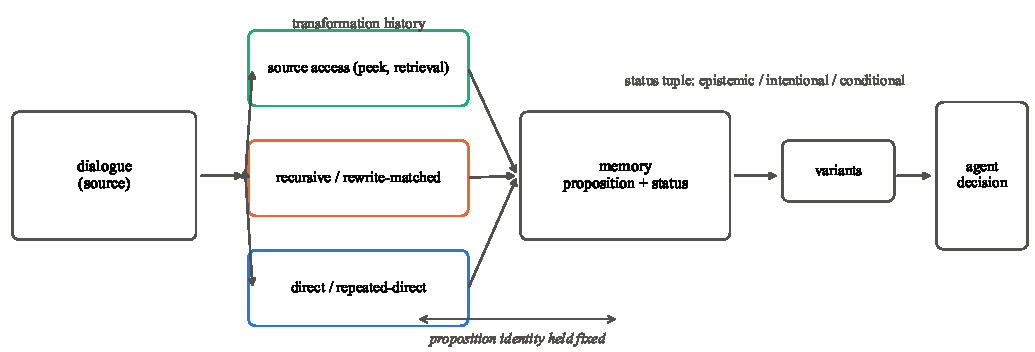
\includegraphics[width=\textwidth]{figures/fig1_design.pdf}
\caption{Design. Paired transformation histories act on the same evidence; the
memory is scored on proposition identity and status; status-only variants drive
a downstream decision.}
\label{fig:design}
\end{figure*}

\subsection{Main result: omission, not distortion}

Of the 330 items, 300 preserve the proposition. The adjudicated distribution is
\st{NO\_DISTORTION} 182, \st{STATUS\_OMISSION} 88, \st{PROPOSITION\_LOSS} 30,
\st{LEGITIMATE\_UPDATE} 27, and \st{UNSUPPORTED\_STATUS\_DISTORTION} 3. Among
the 300 preserved items, 88 are status omissions (29.3\%); unsupported
distortion is 3/330 (0.9\%). The dominant failure is omission, not distortion.

Figure~\ref{fig:omission} shows omission among preserved items by condition.
Direct, repeated-direct, source-peek, and raw are at or below 3.7\%; chained
conditions are 42--54\%. Dimension rates among preserved items are conditional
27.6\%, epistemic 33.0\%, and intentional 27.3\%. An earlier deterministic-cue
result that intentional commitment cues are uniquely vulnerable does not
replicate in these blind labels.

\begin{figure}[t]
\centering
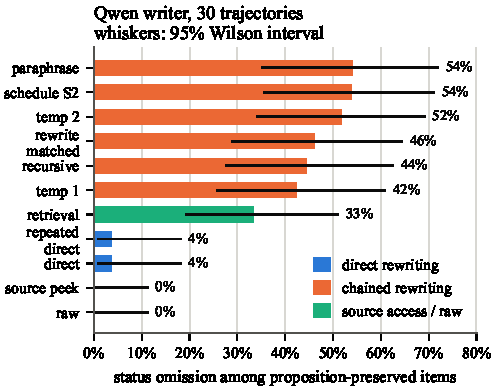
\includegraphics[width=\columnwidth]{figures/fig2_omission.pdf}
\caption{Status omission among proposition-preserved items by condition, with
95\% Wilson intervals. Colors group direct rewriting, chained rewriting, and
source access.}
\label{fig:omission}
\end{figure}

\subsection{Mechanism: chaining, not budget or call count}

We predeclared three mechanism contrasts. Rewrite-matched holds intermediate
budgets constant and recovers the same degradation as the shrinking schedule
(paired omission difference $0.000$ $[-0.167, 0.167]$). Repeated-direct matches
the writer-call count but behaves like direct ($-0.367$ $[-0.567, -0.167]$).
Source-peek, which exposes the original dialogue at every rewrite, removes the
omission ($-0.400$ $[-0.567, -0.233]$). Figure~\ref{fig:mechanism} shows the
three contrasts. The mechanism is therefore repeated re-editing of the writer's
own output, not intermediate budget shrinkage or raw call count. Proposition-loss
differences for these three contrasts are near zero with intervals including
zero, so the omission contrast is not produced by differential proposition loss.
Unsupported distortion has only three events; condition contrasts for it are
uninformative and must not be read as evidence of equivalence.

\begin{figure}[t]
\centering
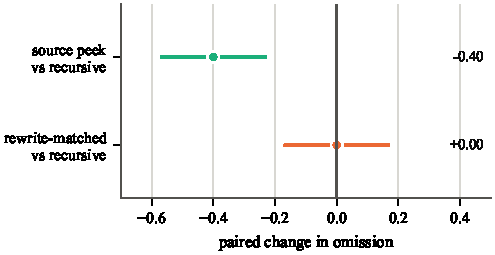
\includegraphics[width=\columnwidth]{figures/fig3_mechanism.pdf}
\caption{Mechanism contrasts on status omission, conditional on proposition
preservation. Error bars are paired bootstrap 95\% intervals.}
\label{fig:mechanism}
\end{figure}

\section{Study 2: Downstream Behavior}

\subsection{Study 2a: synthetic decision task}

Thirty trajectories were paired with four memory variants: present, omitted,
distorted, and no-memory. The agent chooses \st{PROCEED}, \st{CONFIRM},
\st{ABSTAIN}, or \st{OTHER} in a sandboxed task. Evidence supports execution only
for \st{COMMITTED} in the intentional dimension and \st{ESTABLISHED} in the
epistemic dimension; conditional items never support execution because their gold
action is only considering.

Present status produced unauthorized action in 2/30 cases (6.7\%) and
evidence-consistent action in 28/30. Omitted status produced no unauthorized
action (0/30) but only 20/30 evidence-consistent actions: the agent asks instead
of acting. Distorted status produced unauthorized action in 20/30 (66.7\%) and
evidence-consistent action in 0/30. No-memory produced no unauthorized action.
Paired against present, omitted unauthorized is $-0.067$ $[-0.167, 0.000]$ and
evidence-consistent $-0.267$ $[-0.467, -0.067]$; distorted unauthorized is
$+0.600$ $[0.433, 0.767]$ and evidence-consistent $-0.933$ $[-1.000, -0.833]$.
A second agent model (gemma3:12b) reproduces the asymmetry: present 0/30,
omitted 0/30, distorted 20/30 unauthorized.

\subsection{Study 2b: high-stakes authorization bank}

Study 2b is a stricter English authorization bank: 54 scenarios (34
over-commitment, 20 authorized-execution controls) $\times$ 2 request forms
(neutral permission judgment; action) $\times$ 4 memory variants. Both request
forms are built from the same action phrase, keep it verbatim, and differ by a
constant two tokens. The authorization rule states both that the current request
is not evidence of prior authorization and that a memory stating the user
decided, committed, or authorized the action is prior authorization.

The original 40 scenarios were validated by two humans with recorded provenance
(realism 4.11/5 pooled; \emph{only-status-differs} 38/40, $\kappa$ 0.655).
Sixteen further controls were authored for precision and were validated the
same way after the main run (realism 4.97/5 pooled;
\emph{only-status-differs} 15/16, $\kappa$ 1.000); one expansion scenario was
excluded because its distorted variant changes the proposition.
Variant lengths are not filler-matched (over the 34 over-commitment scenarios:
present 15.4 whitespace tokens on average, omitted 10.1, distorted 10.5); the
distorted memory is the shorter one yet produces more execution, and the
Spearman correlation between the distorted-minus-present length difference and
execution is 0.02, so length does not explain the effect.

Table~\ref{tab:auth} reports unauthorized execution on the 34 over-commitment
scenarios for three agent models: the primary local model (gemma3:12b), a second
local model (qwen2.5:7b), and a third, non-local gateway model
(glm-5.3-flash). Present status executes nothing in either form and no-memory
executes nothing in either form for all three models, so every execution in the
omitted and distorted cells requires the memory. \textbf{Distortion is the
robust cross-model harm}: gemma3:12b 24/34 neutral and 10/34 action;
glm-5.3-flash 28/34 neutral and 26/34 action; qwen2.5:7b is floor-limited at
1/34 in each form and is reported as a model-class limitation, not a
replication.

The request-form modulation is model-dependent. For gemma3:12b the
difference-in-differences (action minus neutral) is $-0.429$
$[-0.607, -0.250]$ for distortion and $-0.179$ $[-0.321, -0.036]$ for omission:
asking the agent to act roughly halves the distortion harm and removes the
omission harm. For glm-5.3-flash the same interactions are $-0.059$
$[-0.206, 0.088]$ and $-0.088$ $[-0.206, 0.000]$; neither interval excludes
zero, so the action form does not attenuate either effect on that model. The
safe cross-model claim is therefore the \emph{direction} of the distortion
effect, not its request-form modulation. Excluding six scenarios whose
distortion asserts that the action is already completed leaves the pattern for
gemma3:12b (neutral omitted $+0.179$ $[0.036, 0.321]$; neutral distorted
$+0.679$ $[0.500, 0.857]$; action distorted $+0.250$ $[0.107, 0.429]$).

A ten-scenario analyst-translated Chinese slice reproduces the distortion effect
and its attenuation under the action request for gemma3:12b (7/7 distorted
executions under the permission judgment versus 4/7 under the action request;
difference-in-differences $-0.429$), but with seven items per cell it does not
reproduce the request-dependence of omission over-action
(Supplementary Appendix~F).

\begin{table}[t]
\centering
\small
\setlength{\tabcolsep}{3.2pt}
\begin{tabular}{lccc}
\toprule
 & \multicolumn{2}{c}{unauthorized exec.} & \\
\cmidrule(lr){2-3}
Memory & neutral & action & \\
\midrule
\multicolumn{3}{l}{\emph{gemma3:12b (primary)}} \\
Present & 0/34 & 0/34 \\
Omitted & 5/34 & 0/34 \\
Distorted & 24/34 & 10/34 \\
No memory & 0/34 & 0/34 \\
\addlinespace[2pt]
\multicolumn{3}{l}{\emph{glm-5.3-flash (gateway)}} \\
Present & 0/34 & 0/34 \\
Omitted & 7/34 & 4/34 \\
Distorted & 28/34 & 26/34 \\
No memory & 0/34 & 0/34 \\
\addlinespace[2pt]
\multicolumn{3}{l}{\emph{qwen2.5:7b (floor-limited)}} \\
Present & 0/34 & 0/34 \\
Omitted & 0/34 & 0/34 \\
Distorted & 1/34 & 1/34 \\
No memory & 0/34 & 0/34 \\
\bottomrule
\end{tabular}
\caption{Study 2b: unauthorized execution on the 34 over-commitment scenarios,
v3.1 design, by agent model and request form. All 34 are from the
human-validated scenario set; the 20 authorized controls are not shown here and
the 16 expansion controls were two-human validated after the run (15/16
only-status-differs).}
\label{tab:auth}
\end{table}

By dimension for gemma3:12b, distortion is 16/24 intentional and 8/10
conditional under the neutral form, and 4/24 and 6/10 under the action form;
omission is 3/24 and 2/10 (neutral) and 0 in both (action). Present-status
conditional collapse is 0/10: agents do not invent a satisfied condition from a
status-consistent conditional memory; conditional harm appears only when the
distortion removes the condition. On the 20 authorized controls, present
executes 20/20 (neutral) and 18/20 (action); omitted controls execute 7/20 and
2/20, which is the same defect seen from the correct-action side, not evidence
that omission preserves authorization.

Figure~\ref{fig:behavior} places the two downstream studies side by side and
shows the three-model comparison. Among the local models we tested, only
gemma3:12b passes the action-form control gate; qwen2.5:7b executes one distorted
scenario in each form but fails the gate (10/20), and a third local family also
fails it (9/20). The gateway model passes the gate once one format-only parse
artifact is read semantically (20/20).

\begin{figure*}[t]
\centering
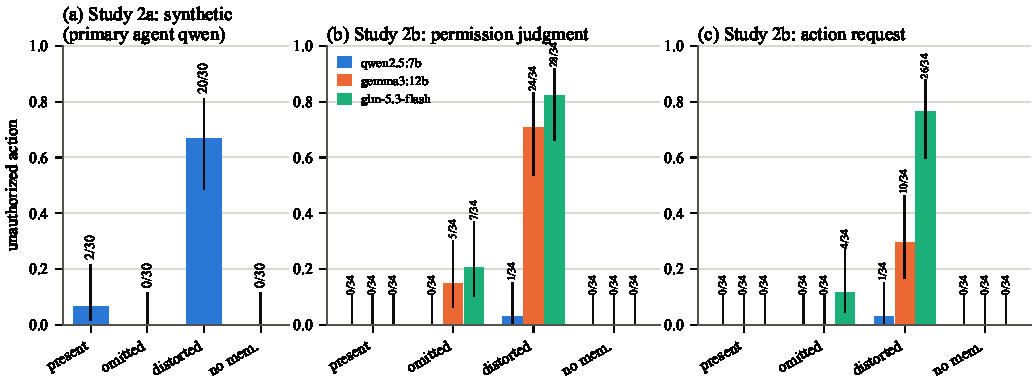
\includegraphics[width=\textwidth]{figures/fig4_behavior.pdf}
\caption{Downstream behavior. (a) Study 2a unauthorized action by variant
(primary agent). (b--c) Study 2b over-commitment unauthorized execution by
memory variant and agent model, for the permission-judgment and action request
forms. Bars are 95\% Wilson intervals.}
\label{fig:behavior}
\end{figure*}

\subsection{Mechanism of unauthorized action}

We coded all 39 over-commitment executions of the primary model from the reason
text. Every distorted execution (34; 24 neutral, 10 action) follows a memory
that states a decision or authorization. Every omission execution (5, all
neutral) turns ``the user mentioned consenting/agreeing/committing'' into ``the
user consented/agreed/committed''; one also treats the conditional clause as
satisfied. No case uses the current request as authorization, and no omission
case executes while acknowledging that the memory lacks a status. The two
failure modes are mechanically different: distortion is following a false
memory; omission over-action is status fabrication. The same coding on the
gateway model (65 executions: 54 D1, 11 O2, 0 O1/O3) reproduces this split. The
coding is post hoc, gold-unblinded, and analyst-performed. A second blind coding
of the same 39 records agrees 39/39 with the analyst (raw 1.00, $\kappa$ 1.00),
but its annotator provenance is unrecorded, so it is not counted as an
independent human rating.

\subsection{Do not pool the downstream tasks}

Study 2a and Study 2b are different task families: a synthetic decision task
with short Chinese templates, and a curated English authorization bank with
positive controls and two request forms. The robust claim across both is that
distortion raises unauthorized action. The omission claim is task- and
request-dependent and must be stated as such. Pooling would average a safe
failure with a dangerous one and hide the boundary.

\section{Mitigation}

Study 3 asks which writer mitigation preserves status at matched budget. The
confirmatory design is a $2\times2$ crossing of prompt (neutral vs status-aware)
and source access (memory-only vs memory plus source) on 30 trajectories, using
the same five-stage chain $220 \to 180 \to 140 \to 120 \to 100$. Generation was
120/120 with zero errors. Budget inflation relative to neutral was $1.05\times$
for status-aware, $1.23\times$ for source access, and $1.38\times$ for the
combination, all below the pre-registered $1.5\times$ flag.

\begin{table}[t]
\centering
\small
\setlength{\tabcolsep}{4pt}
\begin{tabular}{lccc}
\toprule
Condition & Faithful & Omission & Budget \\
\midrule
Neutral & 14/26 & 11/26 & $1.00\times$ \\
Status-aware prompt & 27/30 & 0/30 & $1.05\times$ \\
Source access & 30/30 & 0/30 & $1.23\times$ \\
Status-aware + source & 28/30 & 0/30 & $1.38\times$ \\
\bottomrule
\end{tabular}
\caption{Study 3: faithful status (gold labels) by condition, 30 trajectories;
primary annotator $\kappa$ 0.974 post-adjudication. Remaining items are
unsupported (neutral 1, status-aware 2, combination 1) or ambiguous
(status-aware 1, combination 1); source access has none.}
\label{tab:mitigation}
\end{table}

Source access is the stronger mitigation ($+0.533$ faithful $[0.367, 0.700]$);
the prompt is partial ($+0.433$ $[0.267, 0.600]$); the combination adds nothing
($+0.467$ $[0.300, 0.633]$; interaction $-0.500$ $[-0.667, -0.333]$) and
introduces an escalation pattern in the primary model. Table~\ref{tab:mitigation}
reports the per-condition counts; Figure~\ref{fig:mitigation} compares the
primary and replication writers. The practical recommendation is to expose the
source at rewrite time and treat prompting as a fallback.

The ranking is model-dependent. In the second-writer replication (first 12
pre-registered trajectories), faithful status is direct 11/12, repeated-direct
11/12, source 10/12, status-aware 11/12, combination 12/12, recursive 8/12, and
rewrite-matched 6/12 ($\kappa$ 0.834). The chain effect replicates in direction:
rewrite-matched is the worst condition. But source access alone is weaker in the
second writer (0.83) than in the primary one (1.00), while the prompt and the
combination are at or above the primary values. Report the model boundary, not a
universal mitigation ranking.

\begin{figure*}[t]
\centering
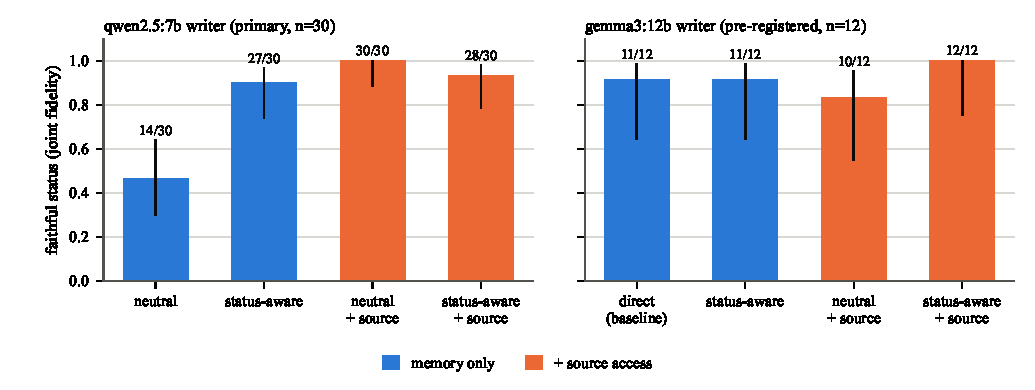
\includegraphics[width=\textwidth]{figures/fig5_mitigation.pdf}
\caption{Faithful status by condition for the primary writer and the
replication.}
\label{fig:mitigation}
\end{figure*}

\section{Real-Dialogue Feasibility and Measurement Attempt}

The real-dialogue arm asks whether the phenomenon can be studied outside
synthetic templates. A rule-based screen over two long-conversation benchmarks,
LoCoMo \citep{locomo} and LongMemEval \citep{longmemeval}, produced 2,135
candidate spans (intentional 1,123, epistemic 981, conditional 31); 725 are
re-mentioned in a later session (34.0\%) and 269 contain a potential change cue
(12.6\%). On semantic reading of a 50-item balanced screen, intentional status
dominates (32/50), epistemic is nearly absent (2/50), and only 4/50 are clearly
consequential for a downstream authorization decision.

The screening rubric itself exposed measurement problems. Two annotators worked
independently, but one used an AI first draft and reviewed every cell, so the
pair is a mixed-provenance diagnostic. Agreement was usable for dimension (0.920
raw / 0.826 $\kappa$) but weak for status-bearing (0.920/0.606) and update
presence (0.840/0.170). A 40-item gold-coding calibration passed status after
third-person adjudication (dimension 1.000/1.000, status 0.975/0.969), but a
45-memory lexical/semantic status-fidelity (LSF/SSF) sheet failed calibration
twice (run 2: LSF 0.800/0.689, SSF 0.756/0.625, proposition identity
0.800/0.607). Proposition identity is the blocker, because memories replace the
target speech act. We therefore scope the real-dialogue arm to feasibility and
gold coding and report the failed LSF/SSF calibration as a measurement lesson
and future work, not as evidence about memory systems
(Supplementary Appendix~E).

\section{Discussion}

\textbf{Two failure modes, two mechanisms.} Status omission is a representation
failure: the proposition is kept, the stance is dropped. Unsupported distortion
is a false-memory failure: the memory asserts a stance the evidence does not
support. They have different behavioral profiles. Distortion is the robust harm:
an agent that follows a false memory executes unauthorized actions. Omission is
the common failure, but it is not uniformly safe.

\textbf{Why ``omission is conservative'' is not a law.} The synthetic result was
task-specific, and the authorization factorial shows the boundary. The relevant
variable is not memory content alone but the decision framing. When the agent is
asked to rule on whether an action is permitted, a bare mention in memory can be
read as authorization and the agent executes; when asked to perform the action,
the same memory may yield a request for confirmation---though, as the gateway
model shows, even that is not guaranteed across models. Papers that report a
single ``status drift'' effect would miss this.

\textbf{Measurement.} Fact recall is not enough. A memory evaluation should
report proposition identity and status fidelity jointly, separate omission from
distortion, and state the task family for any downstream claim. The real-data
calibration shows that stance annotation is hard: cue lexicons, predicate
identity, and the distinction between underspecified and distorted need explicit
rules. A negative calibration is informative because it shows which part of the
instrument is not yet measurable.

\section{Conclusion}

Status fidelity is a distinct measurement target for long-term memory. Chained
rewriting omits the status of a proposition while keeping the proposition;
unsupported distortion is rare in rewriting but dominates downstream behavior
across three model families. In the high-stakes authorization factorial, a
distorted status raised unauthorized execution from 0/34 to 24/34
(gemma3:12b) and 0/34 to 28/34 (glm-5.3-flash) under a permission judgment.
Omission over-action appeared by upgrading a bare mention into a commitment, not
by treating the request as authorization. Omission is common and sometimes safe,
but not a general guarantee, and whether it is safe depends on how the
downstream decision is framed and which model reads the memory. Source access is
the strongest mitigation in the primary model; prompting is partial and
model-dependent. Real-dialogue stance annotation remains an open measurement
problem.

\section*{Limitations}

\begin{itemize}
\item \textbf{Scope and models.} The synthetic study uses templates and local
  7B--12B models plus one gateway model; it is a mechanism study, not a
  model-ranking claim. The Chinese parallel slice is analyst-translated and not
  human-validated. The gateway model's pre-amendment run is reported as a design
  sensitivity, not pooled with the v3.1 estimates.
\item \textbf{Power and multiplicity.} Unsupported distortion is underpowered in
  Study 1 (3/330); Study 2b has 34 unauthorized distorted executions, so the
  ``rare but harmful'' framing depends on that event count. Study 1 evaluates
  ten exploratory conditions with no multiplicity correction. We report
  intervals, not $p$-values.
\item \textbf{Annotation provenance and adjudication.} Human-label provenance is
  unrecorded for the synthetic annotation and adjudication is model-assisted; we
  report those labels as annotator-unspecified, not as independent human
  reliability. All reported $\kappa$ values are post-adjudication. The
  second-writer replication covers 12 trajectories ($\kappa$ 0.834).
\item \textbf{Bank construction.} Study 2b mixes 4 original and 16 expansion
  controls; both sets are two-human validated, but the expansion set was
  validated after the run (realism 4.97, \emph{only-status-differs} 15/16,
  $\kappa$ 1.000), and one scenario is excluded. The scenario list was not
  human-reviewed before the run. Variant lengths are not
  filler-matched; the check is correlational but the direction is conservative.
\item \textbf{Reason coding.} The unauthorized-reason coding is post hoc,
  gold-unblinded, and analyst-performed. A second blind coding agrees 39/39
  (raw 1.00, $\kappa$ 1.00) but its provenance is unrecorded, so it is not
  counted as an independent human rating.
\item \textbf{Real-dialogue arm.} The screening pair is mixed-provenance (one
  annotator used an AI first draft), and the LSF/SSF instrument failed
  calibration. The real-data arm is a feasibility and measurement appendix.
\item \textbf{External validity and ethics.} All downstream decisions are
  sandboxed labels; no real action is executed, scenarios are author-written and
  concern money, health, authorization, and commitments, and nothing here
  licenses deploying a tested model as an authorization gate. The intended use
  is evaluation and mitigation.
\end{itemize}

\bibliographystyle{unsrtnat}
\bibliography{custom}

\end{document}
